We think of an infinity category as a category whose morphism spaces are actually spaces, such that there are coherent higher composition laws. One possible way of modelling such things is using the notion of a simplicial set.

Resources: Emily Riehl's notes on simplicial sets: \url{https://math.jhu.edu/~eriehl/ssets.pdf}

\section{Simplicial sets basics}

\subsection{Definition}

We first define $\Delta$ as the category which has objects $[n]=\{0,1,\dots, n\}$ and morphisms which are order-preserving set maps. 

\begin{definition}{Simplicial set}{Simplicial set}
    A simplicial set is a presheaf on $\Delta$, in other words a functor $$X:\Delta^{op}\rightarrow \Set$$
\end{definition}

We denote $X([n])=X_n$. 

We notice that the category $\Delta$ comes with certain natural maps which generate it: namely, the maps $$\begin{gathered}
    d^i:[n-1]\rightarrow [n], \text{ 'misses i' }\\
    s^i:[n+1]\rightarrow [n], \text{ 'squishes down i, i+1'}
\end{gathered}$$

These operations satisfy the properties $$\begin{gathered}
    d^jd^i = d^id^{j-1}, i<j\\
    s^js^i=s^is^{j+1}, i\leq j\\
    s^jd^i = \begin{cases}
        1, i=j,j+1\\
        d^is^{j-1}, i<j\\
        d^{i-1}s^j, i>j+1
    \end{cases}
\end{gathered}$$

Every map can be factorized using the (co)face and (co)degeneracy maps, and hence we can think of a simplicial set $X$ as a module over the algebra generated by these relations. They define face and degeneracy maps on $X$ as follows: $$d_i = Xd^i:X_n \rightarrow X_{n-1}, s_i = Xs^i:X_n \rightarrow X_{n+1}$$

Sometimes, a simplicial set is drawn as follows: \[\begin{tikzcd}
	{X_0} & {X_1} & {X_2} & \dots
	\arrow[from=1-1, to=1-2]
	\arrow[shift right, from=1-2, to=1-1]
	\arrow[shift left, from=1-2, to=1-1]
	\arrow[shift right, from=1-2, to=1-3]
	\arrow[shift left, from=1-2, to=1-3]
	\arrow[shift left=2, from=1-3, to=1-2]
	\arrow[from=1-3, to=1-2]
	\arrow[shift right=2, from=1-3, to=1-2]
\end{tikzcd}\]

We see that a map of simplicial sets $X\rightarrow Y$, which is a natural transformation, can also be seen as a collection of maps $X_n\rightarrow Y_n$ which commutes with the face and degeneracy maps.

We say that a simplex $x\in X_n$ is \emph{degenerate} if it comes from one of the degeneracy maps. 

\subsection{Yoneda and the standard simplices}

Recall that the Yoneda embedding $$\mathscr{Y}:\calC\rightarrow \Set^{\calC^{op}}, c\mapsto \calC(-,c)$$
is a full and faithful embedding such that $$\Hom(\mathscr{Y}c, F)\simeq F(c)$$

We denote the image under Yoneda of $[n]$ by $\Delta^n$. These are precisely the representable simplicial sets, and every other one can be built from them by what is called the \emph{density theorem}. We see that
$$\mathrm{Hom}_{\mathbf{sSet}}(\Delta^n, X)=X_n$$
More explicitly, the $m$ simplices of $\Delta^n$ are (by the Yoneda embedding) $$\Delta^n_m=\mathrm{Hom}([m],[n])$$

Importantly, the action of the face and degeneracy maps on a morphism $[k]\rightarrow [n]$ is composition on the left: $$[k]\rightarrow [n]\mapsto [k-1]\rightarrow [k]\rightarrow [n]$$or 
$$[k]\rightarrow [n]\mapsto [k+1]\rightarrow [k]\rightarrow [n]$$

The nondegenerate simplices are essentially the injective maps $[m]\rightarrow [n]$. The unique nondegenerate $n$-simplex comes from the identity map. If we identify $x\in X_n$ as a map $x:\Delta^n\rightarrow X$, then $$d_i(x)\in X_{n-1}\leftrightarrow \Delta^{n-1}\xrightarrow{d^i}\Delta^n \xrightarrow{x}X$$

Analogously to how CW complexes are built out of standard simplices, we have the following:
\begin{theorem}{Density theorem}{}
Every simplicial set is a colimit of the standard $n$-simplices: $$\varinjlim_{x\in X_n}\Delta^n \simeq X$$    
\end{theorem}

Essentially, every $x\in X_n$ contributes a $x:\Delta^n\rightarrow X$, but these are glued along in some combinatorial way. The index over which we take the colimit is the category of ends, which has objects $x\in X_n$ for some $n$ and morphisms $f:x\rightarrow y$ precisely when this is induced by some map $[n]\rightarrow [m]$, taking $x$ to $y$. 

\subsection{Nerves, total singular complex and the geometric realization}

\begin{example}{Nerve of a category}{}
    Given a category $\mathcal{C}$, we define a simplicial set $\mathcal{N}\mathcal{C}$ as 
    \begin{itemize}
        \item $\mathcal{NC}_0=\mathrm{ob} \, \mathcal{C}$
        \item $\mathcal{NC}_1=\mathrm{mor}\,\mathcal{C}$
        \item  $\mathcal{NC}_2=$ pairs of composable arrows
        \item ...
    \end{itemize}
    The degeneracy maps send a string of $n$ composable arrows to $n+1$ composable arrows by inserting the identity map somewhere. The face maps compose two consecutive maps. This is a simplicial set, and in fact a quasicategory (we will see what this means in a moment)
\end{example}

Now we consider the geometric realization of a simplicial set.

We first define $$\Delta: \mathbf{\Delta}\rightarrow \mathbf{Top}$$by $\Delta([n])=\Delta_n$, the standard $n$-simplex.  We would like to extend this, via some sort of Kan extension, to a functor on $\sSet$: \[\begin{tikzcd}
    & \sSet \arrow[rd, dotted] &              \\
\mathbf{\Delta} \arrow[ru, "\mathscr{Y}"] \arrow[rr, "\Delta"] &                          & \mathbf{Top}
\end{tikzcd}\]

The density theorem will allow us to do this:

\begin{example}{The geometric realization}{}
    Given a simplicial set $X$ we define $$|X|:= \frac{\bigg(\coprod X_n\times |\Delta^n|\bigg)}{\sim}$$where $|\Delta^n|=\Delta_n$ and the equivalence relation identifies the ith face of $\{x\}\times \Delta_n$ with $d_i(x)\times \Delta_{n-1}$ and also collapses $\{s_i(x)\}\times \Delta_n$ to $\{x\}\times \Delta_{n-1}$. Using the description of Kan extensions and coends, one also realizes this as $$|X|=\int^nX_n\times \Delta_n=\mathrm{colim}\bigg(\coprod_{f}X_m\cdot \Delta_n 
    \substack{\xrightarrow{f_*}\\[-0.9em] \xrightarrow[f^*]{}} \coprod_{[n]} X_n\cdot \Delta_n\bigg)
    $$
    Interestingly, the Kan complexes are determined by their geometric realization, up to homotopy!
    
    \end{example}

This is the left adjoint to the functor $S$ taking a topological space $Y$ to its total singular complex $SY$: given any topological space $Y$, we can define $$SY_n=\mathbf{Top}(\Delta_n, Y)$$as the space of maps from the n-simplex to $Y$. Pre-composition with the maps which insert a zero in some coordinate, or add the i-th and i+1-th coordinates, produce maps which satisfy the simplicial set relations. We get the adjunctions \[\begin{tikzcd}
	\sSet & {\mathbf{Top}}
	\arrow[""{name=0, anchor=center, inner sep=0}, "{|-|}", curve={height=-6pt}, from=1-1, to=1-2]
	\arrow[""{name=1, anchor=center, inner sep=0}, "S", curve={height=-6pt}, from=1-2, to=1-1]
	\arrow["\dashv"{anchor=center, rotate=-90}, draw=none, from=0, to=1]
\end{tikzcd}\]

These in fact form what is called a \emph{Quillen equivalence of model categories}: the homotopy categories of both sides are the same, and the Kan complexes correspond to topological spaces.

This fits into a more general picture: whenever we left Kan extend $F:\mathbf{\Delta}\rightarrow \calE$ via Yoneda, we get a right adjoint $$R:\calE \rightarrow \sSet, Re_n = \calE(F[n],e)$$

These two functors are extremely useful. For example, the classifying space of a group $G$ can be constructed by taking the nerve of the category defined by $G$ and then its geometric realization. Similarly, if one takes the geometric realization of $SY$, then it forms a CW complex whose cellular homology is the same as the singular homology of $Y$: $$C^{\mathrm{cell}}_\bullet(|SY|)\simeq C_\bullet^{\mathrm{sing}}(Y)$$



\begin{example}{Internal homs}{}

We have a functor $$\mathbf{\Delta}\rightarrow \mathbf{sSet}$$ given by taking the product with a fixed $Y$, $F[n]=\Delta^n\times Y$. The Kan extension along the Yoneda embedding is naturally the functor $L=-\times Y$. This has as a right adjoint the functor defined by $$RZ_n=\mathbf{sSet}(\Delta^n\times Y, Z):=[Y,Z]_n$$
The face and degeneracy maps are the ones induced by postcomposition from the ones on $\Delta^n$.
\end{example}

\subsection{Horn fillings and quasicategories}

We study some simplicial subsets of $\Delta^n$. Recall that we have an element $$d^i\in \Delta^n_{n-1}=\mathrm{Hom}([n-1],[n])$$which omits $i$. We think of this as an element in the $n-1$ part of the simplicial set $\Delta^n$. This then generates a subsimplicial set. Note that by Yoneda, the map $d^i$ corresponds to an embedding $$\Delta^{n-1}\rightarrow \Delta^n$$ and we call the image $\partial_i\Delta^n$. 

The union of all the boundaries we call $\partial \Delta^n$ and it can be represented as the subsimplicial set defined as $$(\partial \Delta^n)_m=\{\alpha\in\mathrm{Hom
}([m],[n])|\,\text{not surjective}\}$$Why? Well, note that what the $d^i$ generate is precisely all the morphisms one can get by composing a bunch of morphisms $d^j, s^j$, one of which is $d^i:[n-1]\rightarrow [n]$. But any non-surjective morphism must miss some $i$, so factorizes through one of these $d^i$. The converse is obviously also true: any composition involving $d^i$ is nonsurjective.

Similarly, we can define the i-th horn $$(\Lambda^n_i)[m]=\{\alpha|\,[n]\subsetneq \alpha([m])\cup\{i\}\}$$
or equivalently as the subsimplicial set defined by all faces except the $i-th$ one, since the morphisms generated by composing with anything but the $d^i$ will always hit $i$ and miss something else.

For example, a filling in of $\Lambda^2_1$ would constitute a 2-simplex $\sigma$ such that $d_2\sigma=f, d_0\sigma=g$. 

\begin{definition}{Kan complexes and quasicategories}{}
    A Kan complex is a simplicial set for which every horn admits a filling. An infinity category is a simplicial set $X$ such that any inner horn $i<n$ can be filled.
\end{definition}

\begin{proposition}{Singular chains are Kan complexes}{}
    For a topological space $Y$, its singular chain $SY$ is a Kan complex.
\end{proposition}
\begin{proof}
    By adjunction, we turn the left diagram into the right one, but since $|\Lambda^n_k|$ is a homotopy retract of $|\Delta^n|$, we have a lift.\[\begin{tikzcd}
        & {} & {} \\
        {\Lambda^n_k} & SY & {|\Lambda^n_k|} & Y \\
        {\Delta^n} && {|\Delta^n|}
        \arrow["{\mathrm{adjunction}}", curve={height=-30pt}, squiggly, from=1-2, to=1-3]
        \arrow[from=2-1, to=2-2]
        \arrow[from=2-1, to=3-1]
        \arrow[from=2-3, to=2-4]
        \arrow[from=2-3, to=3-3]
        \arrow[dashed, from=3-1, to=2-2]
        \arrow[dashed, from=3-3, to=2-4]
    \end{tikzcd}\]
    
\end{proof}


\begin{proposition}{Nerves are quasicategories}{}
    The nerve of a category is an infinity category, in which every inner horn has a unique lift.
\end{proposition} 
\begin{proof}
    Essentially, every sequence of composable arrows has unique composition. Or, we can use the fact that the functor $\tau_1$ (the homotopy category) is adjoint to the nerve functor.
\end{proof}

We see then that all usual categories sit inside the quasicategories, but have unique compositions. An infinity category can be thought of as a normal category, but where composition laws are not uniquely defined: there are higher relations among them! We will see, though, that even though compositions are not uniquely defined, they still form a contractible set, so in homotopical terms is still a point.

\begin{definition}{Homotopy equivalence}{}
    Suppose $f,g\in X_1$ are morphisms from $a$ to $b$. We have different relations of equivalence $f\sim_a g, f\sim_b g, g\sim_a f, g\sim_b f$ when there is a triangle filling in $f,g$ and an identity morphisms. These are all equivalent when $X$ is a quasicategory.
\end{definition}

\section{Towards the infinity category of spaces}

The aim of this chapter is two-fold. First, we introduce functor categories, inner fibrations and mapping spaces. Then, we use the homotopy coherent nerve construction and apply it to the simplicially enriched category of Kan complexes to produce the infinity category of spaces.

\subsection{Functor categories}

Recall that we have an internal hom $$\inHom(X,Y)_n=\Hom_{\sSet}(X\times \Delta^n,Y)$$So for an infinity category $C$ and a simplicial set $K$, we define $$\mathrm{Fun}(K,C):=\inHom(K,C)$$

Some examples of functor categories: \begin{itemize}
    \item $\Fun(\Delta^0,C)\simeq C$
    \item $\Fun(\Delta^1,C)$ is the arrow category
    \item $\Fun(\Delta^1\times \Delta^1, C)$ are the commutative squares in $C$, as follows: we have $2$-simplices such that $d_1(\sigma)=d_1(\tau)$. 
\end{itemize} 

To clarify the last point: the product $\Delta^1 \times\Delta^1$ has $4$ $0$-simplices $(0,0), (0,1), (1,0), (1,1)$. The $1$ simplices are pairs of $1$ simplices of $\Delta^1$, which are enumerated by $\{id, 0,1\},$ the identity being the nondegenerate one. However, whilst $0\times 0, 0\times 1, 1\times 0, 1\times 1$ are degenerate (come from the zero simplices by precomposing with $\Delta^1 \rightarrow \Delta^0$), the ones where we multiply with $id$ are not and there are five of them: $id\times id$ being the diagonal, the rest being the sides of a square. The only nondegenerate $2$-simplices come from the different degeneracy maps $[2]\rightarrow [1]$, which give the two triangles. These 2-simplices witness the fact that the top and bottom 'compositions' are the same!

\begin{figure}[H]
    \centering
        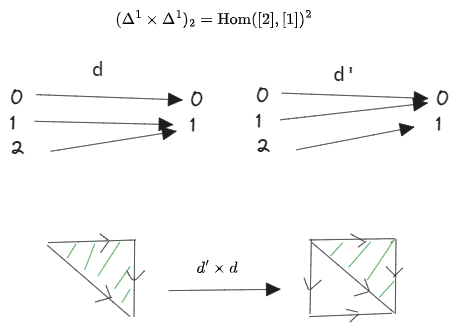
\includegraphics[scale=0.5]{Simplices of simplicial square.png}
        \caption{Nondegenerate 2-simplex}
    \end{figure}

%More precisely, given $f,g\in\Fun(K,C)_0= \Hom_{\sSet}(K,C)$ a natural transformation should be $q\in \Fun(K,C)_1=\Hom_{\sSet}(K\times \Delta^1,C)$ so that $q$ is a natural isomorphism if $q(id_k, id_{\Delta^1}):f(k)\rightarrow g(k)$ is an isomorphism pointwise. This is not entirely obvious! (the identity $id_{\Delta^1}$ is just the map $[0]\rightarrow [1]$).
\begin{definition}{Equivalence of infinity categories}{}
    Let $f:C\rightarrow D$ be a functor between infinity categories. This forms an equivalence if it is an isomorphism in $\Fun(C,D)$, i.e. $\exists g:D\rightarrow C$ so that $f\circ g \simeq id, g\circ f\simeq id$. 
\end{definition} 


This is weaker than a natural isomorphism! For nerves, it means equivalence of 1-cats. For spaces, it means a weak homotopy equivalence. For infinity cats, it means ''fully faithful and essentially surjective''.

Recall: $C$ being an infinity category is equivalent to $$\Hom_{\sSet}(\Delta^n,C)\rightarrow \Hom_{\sSet}(\Lambda^n_i,C)$$being a surjection of sets of outer hom. But if we think of internal hom instead we actually get the equivalent statement that$$\inHom (\Delta^n,C)\rightarrow \inHom (\Lambda^n_i,C)$$is an epimorphism of simplicial sets! Even more is true: this turns out to be a trivial Kan fibration.

We now turn to the claim that when $X$ is an infinity category, then so is $\Fun(K,X)$. The idea is as follows: want to show inner horns extend to n-simplex. By definition, the inner hom is adjoint to the product with $K$, this is equivalent to a map $$\Lambda^n_i\rightarrow \inHom(K,C)\leftrightarrow \Lambda^n_i\times K\rightarrow C$$ and extending it to $\Delta^n\times K$. We add in the structure map to the terminal object: $$\begin{CD}\Lambda^n_i\times K @>>>C \\ @VVV @VVV \\ \Delta^n\times K @>>> \Delta^0\end{CD}$$

We seek a diagonal lift in this problem. 

\begin{definition}{Inner fibrations and inner anodyne maps}{}
 An inner fibration is a map $p:X\rightarrow Y$ with the right lifting property with respect to inner horns, i.e. every diagram like this has a lift: $$\begin{CD}\Lambda^n_i @>>>X \\ @VVV @VVpV \\ \Delta^n @>>> Y\end{CD}$$
 In this sense, an infinity category is just an inner fibration $C\rightarrow \Delta^0$. An inner anodyne map is a map $q:A\rightarrow B$ with the left lifting property with respect to inner fibrations.
\end{definition}

\begin{example}{Functors to nerves}{}
    Any functor $\calC \rightarrow ND$ from a quasicategory to a nerve is an inner fibration. First, let $f:\Lambda^n_i\rightarrow \calC$ be the top arrow. \[\begin{tikzcd}
        {\Lambda^n_i} & \calC \\
        {\Delta^n} & ND
        \arrow["f", from=1-1, to=1-2]
        \arrow[from=1-1, to=2-1]
        \arrow["g", from=1-2, to=2-2]
        \arrow["{\tilde{f}}", dashed, from=2-1, to=1-2]
        \arrow[from=2-1, to=2-2]
    \end{tikzcd}\]
    We see that the composition $g\circ f$ has a unique lift to $ND$ which is the bottom map, since nerves admit unique lifts. On the other hand, since $\calC$ is an infinity category, there is some lift $\tilde{f}:\Delta^n \rightarrow \calC$. The reason this commutes with the bottom arrow is because $g\circ\tilde{f}\circ \iota = g\circ f$ satisfies the uniquely defining property of the map $\Delta^n\rightarrow ND$. 
    
\end{example}

\begin{definition}{Trivial Kan fibration}{}
    A map $p:X\rightarrow Y$ is a trivial Kan fibration if it has the right lifting property with respect to all inclusions of simplicial sets. These are obviously a subset of the inner fibrations. They also admit sections, by taking the inclusion $\emptyset \rightarrow Y$ and the identity map $Y\rightarrow Y$. 
\end{definition}

The Kan fibrations form the \emph{fibrations in the Quillen model structure}, and the monomorphisms form the cofibrations. Trivial Kan fibrations are stable under pullbacks, by using UMP for fiber products. 

So it amounts to showing that $\Fun(K,-)$ preserves inner fibrations, which is also equivalent to the fact that inner anodyne maps are stable under $-\times K$. This is a standard result in the literature. We mention the theorem which allows such arguments to work (Theorem 1.3.37 in Markus Land's book):

\begin{theorem}{Stability of inner fibrations}{Stability of inner fibrations}
    Suppose we are given maps $f:X\rightarrow Y, \iota:A\rightarrow B$ of simplicial sets. This induces a diagram $$\begin{CD}
        \Fun(B,X) @>>> \Fun (A,X)\\
        @VVV @VVV\\
        \Fun(B,Y) @>>> \Fun(A,Y)
    \end{CD}$$
    and hence a map $$\langle \iota ,f \rangle:\Fun(B,X)\rightarrow \Fun(B,Y)\times_{\Fun(A,Y)}\Fun(A,X)$$

    If $f$ is an inner fibration an $\iota$ a monomorphism, then $\langle \iota, f \rangle$ is an inner fibration. If $\iota$ is anodyne, then $\langle \iota, f \rangle$ is trivial.
\end{theorem}

\begin{corollary}{Corollary}{}
    When $A=\emptyset,B=K, X=X, Y=\Delta^0$ we see that $X$ being an infinity category implies that $\Fun(K,X)$ is also an infinity category. Moreover, if $X$ is a Kan complex, then so is $\Fun(K,X)$.
    
\end{corollary}


\begin{lemma}{Equivalent condition for being a quasicategory}{Equivalent condition for being a quasicategory}
    Let $X$ be a simplicial set. Then TFAE:
    \begin{itemize}
        \item $X$ is an $\infty$-category
        \item For every inner anodyne map $i:A\rightarrow B$, the induced map $i^*:\Fun(B,X)\rightarrow \Fun(A,X)$ is a trivial Kan fibration.
        \item $\Fun(\Delta^2,X)\rightarrow \Fun(\Lambda^2_1,X)$ is a trivial Kan fibration.
    \end{itemize}
\end{lemma}

\begin{proof}
    For $(1)\implies (2)$, we use the theorem \ref{th:Stability of inner fibrations}. Namely, we put $Y=\Delta^0$ and we then see that $$\Fun(A,X)\times_{\Fun(A,\Delta^0)}\Fun(B,\Delta^0)\simeq \Fun(A,X)$$: the fiber product informally consists of pairs $f:A\rightarrow X, g:B\rightarrow \Delta^0$ such that the following commutes: $$\begin{CD}
        A @>f>> B \\
        @VVV @VVV\\
        B @>>g> \Delta^0
    \end{CD}$$
    But $f$ can be lifted to $\tilde{f}$ since $A\rightarrow B$ is inner anodyne which determines $g$. So the theorem says that $$\Fun(B,X)\rightarrow \Fun(A,X)$$ is a trivial Kan fibration. This immediately implies $(3)$. 
    
    Finally, to show $(3)\implies (1)$, $X$ to be an infinity category, we must verify that $X\rightarrow \Delta^0$ satisfies the extension property for inner anodynes. We need to appeal to the fact that the inner anodyne maps are generated by all maps of the form $[K\hookrightarrow L] \boxtimes [\Lambda^2_1 \rightarrow \Delta^2]$, where $\boxtimes$ refers to the induced map from the pushout as in the diagram: \[\begin{tikzcd}
        {K\times \Lambda^2_1} & {K\times \Delta^2} \\
        {L\times \Delta^2} & pushout \\
        && {L\times \Delta^2}
        \arrow[from=1-1, to=1-2]
        \arrow[from=1-1, to=2-1]
        \arrow[from=1-2, to=2-2]
        \arrow[from=1-2, to=3-3]
        \arrow[from=2-1, to=2-2]
        \arrow[from=2-1, to=3-3]
        \arrow[dashed, from=2-2, to=3-3]
    \end{tikzcd}\]

    In this case, we can think of the pushout as the intersection, which is just $K\times \Lambda^2_1$ when $K\hookrightarrow L$ is a monomorphism. So the required extension property is reduced to the diagram: \[\begin{tikzcd}
        & {} && {} \\
        {K \times \Lambda^2_1} & X && K & {\Fun(\Lambda^2_1, X)} \\
        {L \times \Delta^2} & {\Delta^0} && L & {\Fun(\Delta^2, X)}
        \arrow["adjunction", curve={height=-30pt}, squiggly, from=1-2, to=1-4]
        \arrow[from=2-1, to=2-2]
        \arrow[from=2-1, to=3-1]
        \arrow[from=2-2, to=3-2]
        \arrow[from=2-4, to=2-5]
        \arrow[from=2-4, to=3-4]
        \arrow[from=2-5, to=3-5]
        \arrow["{?}"{description}, dashed, from=3-1, to=2-2]
        \arrow[from=3-1, to=3-2]
        \arrow["{?}"{description}, dashed, from=3-4, to=2-5]
        \arrow[from=3-4, to=3-5]
    \end{tikzcd}\]
    But by assumption, the right vertical is a trivial Kan fibration, so has the lifting property for all monomorphisms. 
\end{proof}

With this lemma, we can show that the space of compositions is contractible, one of our original aims:

\begin{corollary}{Space of compositions is contractible}{}

Suppose $(g,\bullet,f):\Lambda^2_1\rightarrow C$ is a pair of composable arrows in an infinity category. Then the simplicial set of fillers which are lifts to $\Delta^2$ is the pullback $$\begin{CD} \mathrm{Comp}(f,g)@>>> \Fun(\Delta^2,C)\\ @VVV @VVV \\ \Delta^0 @>>> \Fun(\Lambda^2_1,C)\end{CD}$$
which is a subsimplicial set of $\inHom(\Delta^2,C)$ and this simplicial set is contractible: it is a Kan complex and is weakly homotopy equivalent to $\Delta^0$. \end{corollary}
\begin{proof}
    By the previous theorem, the right vertical arrow is a trivial Kan fibration. Hence, its pullback to $\Delta^0$ is a trivial Kan fibration.
\end{proof}

Generalization: recall that the spine $\mathrm{Sp}_n$ is generated by adjacent edges in $\Delta^n$ and the inclusion is inner anodyne. Hence $$\inHom(\Delta^n,C)\rightarrow \inHom(\mathrm{Sp}_n,C)$$is a trivial Kan fibration. A map from the spine is a sequence of n composable morphisms. Hence we can apply the same argument to show that the space of n-compositions is contractible.

\subsection{Mapping spaces}
With the tools from the previous section, we are ready to define the mapping spaces between two objects in an infinity category.

\begin{definition}{Mapping space}{}
    Given an infinity category $C$, we have a pullback diagram where we evaluate at the two endpoints.  $$\begin{CD} \mathrm{Map}(c,d) @>>> \mathrm{Fun}(\Delta^1, C)\\ @VVV @VVV \\ \Delta^0 @>>> C\times C\end{CD}$$The resulting space $\mathrm{Map}(c,d)$ is a simplicial set, indeed a Kan complex! This is because we can think of $C\times C=\mathrm{Fun}(\partial \Delta^1, C)$ and $\partial \Delta^1 \hookrightarrow \Delta^1$ is inner anodyne, implying by \ref{lemma:Equivalent condition for being a quasicategory} that the right vertical map is a trivial Kan fibration.
\end{definition}


Example: the loop space $\Omega(X)=\mathrm{Map}_X(x,x)$. 

We can see that there is a morphism between two $f,g:c\rightarrow d$ if and only if $f\simeq g$, since basically we have to fill in a square which restricts to $f,g$ on the sides and the identity maps on the top and bottom, since $\Delta^1_0$ has degeneracy maps which have $s(c)=id_c$ and $s(d)=id_d$.

\begin{definition}{Fully faithful functors}{}
    $F:C\rightarrow D$ is fully faithful if, for every $c,d\in C$, the induced map on mapping spaces is a homotopy equivalence: $$\mathrm{Map}(c,d)\xrightarrow{f} \mathrm{Map}(Fc,Fd)$$ 
\end{definition}


Note that this is not a property of the homotopy category! Take $X$ to be a noncontractible, simply-connected space. The canonical map $X\rightarrow \Delta^0$ induces an equivalence on homotopy categories! So, in a way, the homotopy category only sees the first homotopy group, whereas the full infinity groupoid sees everything.

Similarly, we can define essential surjectivity. For spaces, this should be a surjection on $\pi_0$. 

In particular, a map of spaces is ess. surj and fully faithful iff it is a homotopy equivalence.

\begin{proposition}{Proposition}{}
    $F$ is ess surj and fully faithful iff it is an equivalence.
\end{proposition}

\begin{proof}
    Want to reduce this to a question about spaces. Use the following trick: an functor is an equivalence iff it induces isomorphisms on $\mathrm{Fun}(K,C)^{core}\rightarrow \mathrm{Fun}(K,D)^{core}$. Restrict attention to $K=\Delta^1$ first.  Look at evaluation diagram: $$\begin{CD} \mathrm{Fun}(\Delta^1,C) @>>> \mathrm{Fun}(\Delta^1, D)\\ @VVV @VVV \\ C\times C @>>> D\times D\end{CD}$$The vertical arrows are Kan fibrations. The fibers are mapping spaces $\mathrm{Map}(c,c')$ and then we just use the fact that the functor is fully faithful.
\end{proof}

\subsubsection{Subcategories}
Suppose we have a subcategory of the homotopy category of an infinity category $C$. Form a pullback using the nerve construction: 

$$\begin{CD} C' @>>> C\\ @VVV @VVV \\ N(h(C)') @>>> N(h(C)) \end{CD}$$

This is the subcategory of $C$ spanned by $h(C)'$.  This is an infinity category, which can be checked by using the criterion.

\begin{definition}{Cores}{}
    The core of an infinity category is the subcategory spanned by the core of $h(C)$, i.e. the subcategory spanned by isomorphisms. This is the maximal infinity groupoid in $C$.

\end{definition}

\subsubsection{Compositions}

Suppose we have three objects $c,d,e\in C$. Can define a triple mapping space, by instead using $\Delta^2$. 

$$\begin{CD} \mathrm{Map}(c,d,e) @>>> \mathrm{Fun}(\Delta^2, C)\\ @VVV @VVV \\ \Delta^0 @>>> C\times C\times C\end{CD}$$

This has projection maps to the usual mapping spaces. Then $$\mathrm{Map}(c,d,e)\rightarrow \mathrm{Map}(d,e)\times \mathrm{Map}(c,d)$$is a trivial Kan fibration. The fiber is the space of compositions, which is contractible. We thus have a homotopy inverse section i.e. a choice of composition. But this is not well-defined, but only unique up to homotopy. Uses general fact that the sections of a Kan fibration form a contractible set.

*Exercise:* define the simplicial set of sections of a trivial Kan fibration and show it is contractible.

Basically, the idea is that trivial Kan fibrations are stable under $\mathrm{Fun}$ and hence we can form a pullback $$\begin{CD}\Gamma(Y,X)@>>> \mathrm{Fun}(Y,X)\\ @VVV @VVpV \\ \Delta^0 @>>id> \mathrm{Fun}(Y,Y)\end{CD}$$





\subsection{The homotopy coherent nerve}
In this section, we describe an adjunction between the simplicial sets and simplicially enriched categories in the form of the coherent nerve and the thickening functor. This also forms a Quillen equivalence between Quillen's model structure on $\sSet$ and Segal's model structure on 
We have a 'thickening' functor $$\mathfrak{C}:\mathbf{\Delta}\rightarrow \mathbf{sCat}$$
This can be left Kan extended to a functor on simplicial sets, and has an adjoint called the \emph{homotopy coherent nerve}.

Suppose we have a 1-category $C$ and some class of morphisms $W\subset C_1$. Can form a universal localization category $C[W^{-1}]$ which inverts these maps, but this is not well-behaved. The correct thing to define is a actually an infinity category. 

The construction is involved.

Suppose $0\leq i\leq j$ . Denote by $P_{i,j}$ to be the set of subsets $$P_{i,j}=\{I\subset \{i,...,j\}| i,j\in I\}$$partially ordered by inclusion. If $i>j$ define this to be empty. 

Define $$\mathfrak{C}[\Delta^n]:=\begin{cases}0,1,...,n \text{ as objects}\\\inHom(i,j)=N(P_{i,j}) \end{cases}$$This is a thickening of $\Delta^n$. It is a simplicial category, i.e. a category enriched over simplicial sets. Composition is defined by taking unions of subsets. 

We can extend this functor to $\sSet$ by using e.g. the density theorem and this will be a Kan extension along Yoneda. This defines a functor $\mathfrak{C}$.


\begin{definition}{Spc}{}
    We define a simplicial set whose n-simplices are $$Spc _n:=\Hom_{\mathrm{sCat}}(\mathfrak{C}\Delta^n, \mathrm{Kan})$$
    
    where Kan is the simplicial category of Kan complexes with inner homs as morphisms. This is the homotopy coherent nerve $N(\mathrm{Kan})$, where $N(C)$ is defined analogously, if $C$ is a simplicial set whose inner homs are all Kan. This means that the homotopy coherent nerve is right adjoint to $\mathfrak{C}$. 
\end{definition}

The zero simplices are just the Kan complexes. The 1-simplices are maps of Kan complexes (functors). The first interesting thing is the 2-simplices: an element consists of the following data $$\begin{gathered}f:X\rightarrow Y\\ g:Y\rightarrow Z\\ h:X\rightarrow Y\\ g\circ f\simeq h\end{gathered}$$

\begin{theorem}{Theorem}{}
    The homotopy coherent nerve forms an infinity category and there is a canonical htpy equivalence $$\inHom(X,Y)\simeq \mathrm{Map}_{N\mathcal{C}}(X,Y)$$
\end{theorem}
\begin{proof}
    By adjunction, the lifting diagram corresponds to one involving $\mathfrak{C}[\Lambda^n_i]$, $\mathfrak{C}[\Delta^n]$ and $\mathcal{C}$. These are basically the same except how to extend it to $\inHom(0,n)$. But since $\mathcal{C}$ is locally Kan, this is possible.
\end{proof}

*Example:* the infinity category of quasicategories has objects infinity cats and hom-sets $\mathrm{Fun}(C,D)^\simeq$. We get $\mathrm{Cat}_\infty=N(\mathrm{qCat})$. 

\subsubsection{Infinity Yoneda}

We have a non-unique but contractible choice of compositions, which makes it hard to create a functorial assignment $$\mathrm{Map}(c,d)\rightarrow \mathrm{Map}(c',d)$$

\begin{definition}{Opposite of an infinity category}{}
    The opposite of an infinity category $C:\Delta^{op}\rightarrow \mathrm{Set}$ is given by precomposing with the opposite map on $\Delta$. This is still an infinity category, since $\Lambda^n_i$ just becomes $\Lambda^n_{n-i}$.  
\end{definition}


Presheaves on infinity categories
$$\mathcal{P}(C):=\mathrm{Fun}(C^{op}, Spc)$$
